% Compile using: TEXINPUTS=minted/source: xelatex -shell-escape slides.tex
\documentclass[14pt,compress,english,utf8,t]{beamer}

\usepackage{etex}

\usepackage[english]{babel}

\usepackage{xspace}
\usepackage{ragged2e}

\makeatletter
\ifbeamer@draftmode
\usepackage{verbatim}
\newcommand{\inputminted}[2]{\verbatiminput{#2}}
\else
\usepackage{minted}
\setminted{linenos}
\fi
\makeatother

\usepackage[protrusion=true,expansion=false]{microtype}

\usepackage{fontspec}
\newfontfamily\DejaSans{DejaVu Sans}

\title[
  \raisebox{-0.3mm}{\DejaSans ☺} Perl 6 is out for your enjoyment
  \raisebox{-0.3mm}{\DejaSans ☺}
]{\raisebox{-0.3mm}{\DejaSans ☺} Perl 6 \raisebox{-0.3mm}{\DejaSans ☺} \\
  is out for your enjoyment
}
\author[Ingo Blechschmidt]{\small Ingo Blechschmidt}
\institute{32th Chaos Communication Congress}
\date[December 30th, 2015]{\small December 30th, 2015}

\usetheme{Warsaw}
\usecolortheme{seahorse}
\definecolor{mypurple}{RGB}{150,0,255}
\setbeamercolor{structure}{fg=mypurple}
\usefonttheme{serif}
\usepackage{fontspec}
\defaultfontfeatures{Mapping=tex-text}
\setmainfont{Linux Libertine O}
\useinnertheme{rectangles}
\setbeamercovered{invisible}

\setbeamertemplate{title page}[default][colsep=-1bp,rounded=false,shadow=false]
\setbeamertemplate{frametitle}[default][colsep=-2bp,rounded=false,shadow=false,center]

\setbeamertemplate{navigation symbols}{}
\setbeamertemplate{headline}{}

\newcommand*\oldmacro{}%
\let\oldmacro\insertshorttitle%
\renewcommand*\insertshorttitle{%
  \oldmacro\hfill\insertframenumber\,/\,\inserttotalframenumber\hfill}

\newcommand{\hil}[1]{{\usebeamercolor[fg]{item}{\textbf{#1}}}}

\newcommand{\atpos}[1]{%
  \begin{tikzpicture}[remember picture, overlay]%
    \node[anchor=south east] at (current page.south east) {#1};
  \end{tikzpicture}%
}

\newcommand{\centeredpar}[2]{%
  \begin{center}
    \colorbox{white}{\parbox{#1\textwidth}{%
      #2%
    }}%
  \end{center}%
}

\newcommand{\sourcedquote}[4]{%
  ``#1''\par%
  {\raggedleft -- #2, #3, \href{#4}{\underline{link}}\par}%
}

% Gonzalo Medina, http://tex.stackexchange.com/a/228198
\makeatletter
\def\Mdescription#1{%
  \advance\beamer@descdefault by \labelsep%
  \list
  {}
  {\labelwidth\beamer@descdefault%
  \leftmargin\beamer@descdefault%
  \let\makelabel\beamer@descriptionitem
  \settowidth\labelwidth{\beamer@descriptionitem{#1}}%
  \setlength\leftmargin{\labelwidth}% 
  \addtolength\leftmargin{\labelsep}%
  }%
  \beamer@cramped%
  \raggedright
  \beamer@firstlineitemizeunskip%
}
\def\endMdescription{\ifhmode\unskip\fi\endlist}
\long\def\beamer@descriptionitem#1{%
  \def\insertdescriptionitem{#1}%
  {\usebeamertemplate**{description item}}\hfil}
\makeatother

\setbeameroption{show notes}
\setbeamertemplate{note page}[plain]

\begin{document}

\begin{frame}
  \titlepage

  \vspace*{-1em}
  \begin{center}
    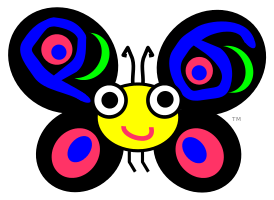
\includegraphics[scale=0.40]{images/camelia}
  \end{center}
\end{frame}

\begin{frame}[plain,c]
  \hspace*{-0.4cm}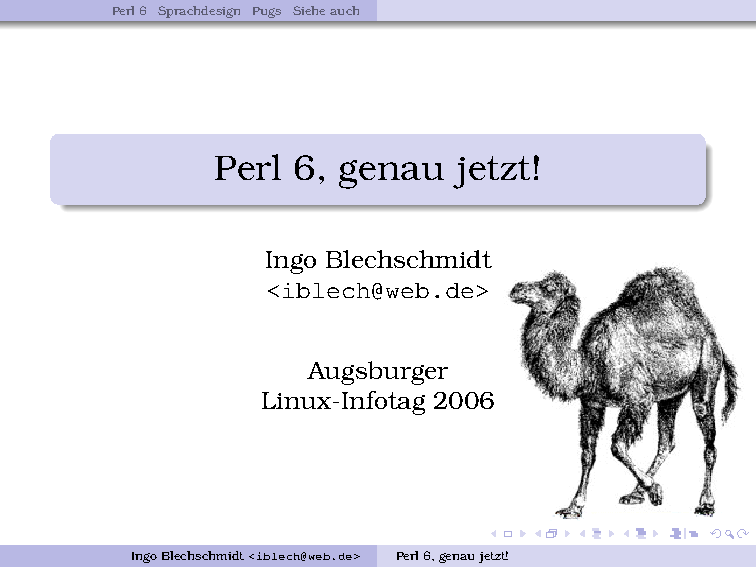
\includegraphics[page=1,scale=0.9]{images/Perl6_LIT_2006.pdf}
\end{frame}

\begin{frame}[plain,c]
  \centering
  
\includegraphics[scale=0.6]{images/happy-camel.jpeg}
  \par
\end{frame}

\begin{frame}[plain,c]
  \centering
  
\includegraphics[scale=0.4]{images/applause}
  \par
\end{frame}

\begin{frame}[fragile]\frametitle{Basic control flow and operators}
  \begin{minted}{perl}
my $name = prompt("What's your name?");
say "Hello $name!";
# or: "Hello $name!".say;

for 0..3 -> $i {
    say "Day $i of congress was great!";
}

say "1 * 2 * 3 * 4 * 5 * 6 is:";
say [*] 1..6;

say (1,2,3) >>+<< (4,5,6);  # (5 7 9)
  \end{minted}
\end{frame}

\begin{frame}[fragile]\frametitle{Object-orientation}
  \begin{minted}{perl}
class SmilingCat is Cat {
    has Num $.smiling-power = 9000;
    has Str $.name where { $^n eq uc $^n };
    # only uppercase names allowed

    method smile(Person $rcpt, Bool $jump?) {
        say "Hello $rcpt!";
        say "I'm jumping!" if $jump;
        $rcpt.happiness += $.smiling-power;
    }
}
  \end{minted}
\end{frame}

\begin{frame}[fragile]\frametitle{Rules}
  \small
  \begin{minted}{perl}
grammar URL {
    rule  TOP   {
        <proto> '://' <host> '/' <path>
    }
    token proto { 'https' | 'ftps' }
    rule  host  { [<domain> '.'?]+ }
    # ...
}

if my $ast = URL.parse("https://a.org/b") {
    # do something with the parse tree $ast
}

# NB: Rules are used in the compiler itself,
# to parse Perl 6 source code.
  \end{minted}
\end{frame}

\renewcommand{\b}{\hil{\textbullet}\xspace}

\begin{frame}\frametitle{\raisebox{-0.3mm}{\DejaSans ☺} Perl 6 is out for your enjoyment \raisebox{-0.3mm}{\DejaSans ☺}}
  {
    \centering
    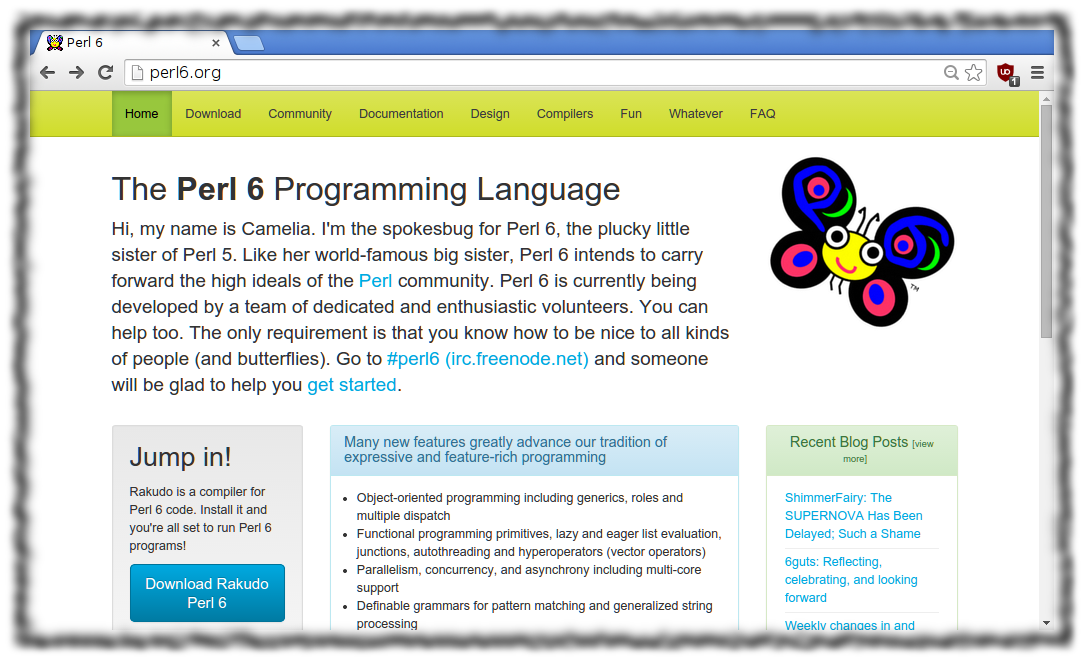
\includegraphics[width=0.7\textwidth]{images/perl6org}
    \par
  }

  \vfill
  \justifying
  \small
  modern \b expressive \b reimagination of Perl 5 \b
  not source-level compatible to Perl~5 \b
  full interop with Perl~5 \b
  gradually typed \b
  multi-paradigmatic \b dramatically overhauled regexes \b
  fully Unicode-aware \b vast meta-programming abilities \b
  implementations decoupled from specification
  \par
\end{frame}

% http://www.impactlab.net/wp-content/uploads/2010/09/Happy-Camel-672.jpg
% http://cdn.theatlantic.com/static/mt/assets/science/bender-applause_medium.gif

\end{document}

\begin{Verbatim}[commandchars=\\\{\}]
\PYGdefault{n}{class} \PYGdefault{n}{SmilingCat} \PYGdefault{n}{is} \PYGdefault{n}{Cat} \PYGdefault{p}{\PYGdefaultZob{}}
    \PYGdefault{n}{has} \PYGdefault{n}{Num} \PYGdefault{n+nv}{\PYGdefaultZdl{}}\PYGdefault{n+nv}{.smiling-power} \PYGdefault{o}{=} \PYGdefault{l+m+mi}{9000}\PYGdefault{p}{;}
    \PYGdefault{n}{has} \PYGdefault{n}{Str} \PYGdefault{n+nv}{\PYGdefaultZdl{}}\PYGdefault{n+nv}{.name} \PYGdefault{n}{where} \PYGdefault{p}{\PYGdefaultZob{}} \PYGdefault{n+nv}{\PYGdefaultZdl{}}{\PYGdefaultZca{}}\PYGdefault{n+nv}{n} \PYGdefault{o+ow}{eq} \PYGdefault{n+nb}{uc} \PYGdefault{n+nv}{\PYGdefaultZdl{}}\PYGdefaultZca{}\PYGdefault{n+nv}{n} \PYGdefault{p}{\PYGdefaultZcb{};}
    \PYGdefault{c+c1}{\PYGdefaultZsh{} only uppercase names allowed}

    \PYGdefault{n}{method} \PYGdefault{n}{smile}\PYGdefault{p}{(}\PYGdefault{n}{Person} \PYGdefault{n+nv}{\PYGdefaultZdl{}rcpt}\PYGdefault{p}{,} \PYGdefault{n}{Bool} \PYGdefault{n+nv}{\PYGdefaultZdl{}jump}\PYGdefault{p}{?)} \PYGdefault{p}{\PYGdefaultZob{}}
        \PYGdefault{n}{say} \PYGdefault{l+s}{"Hello \PYGdefaultZdl{}rcpt!"}\PYGdefault{p}{;}
        \PYGdefault{n}{say} \PYGdefault{l+s}{"I'm jumping!"} \PYGdefault{k}{if} \PYGdefault{n+nv}{\PYGdefaultZdl{}jump}\PYGdefault{p}{;}
        \PYGdefault{n+nv}{\PYGdefaultZdl{}rcpt}\PYGdefault{o}{.}\PYGdefault{n}{happiness} \PYGdefault{o}{+=} \PYGdefault{n+nv}{\PYGdefaultZdl{}}\PYGdefault{n+nv}{.smiling-power}\PYGdefault{p}{;}
    \PYGdefault{p}{\PYGdefaultZcb{}}
\PYGdefault{p}{\PYGdefaultZcb{}}
\end{Verbatim}
